\documentclass[tikz, border=0.5cm]{standalone}
\usetikzlibrary{automata, arrows.meta, positioning}
\begin{document}
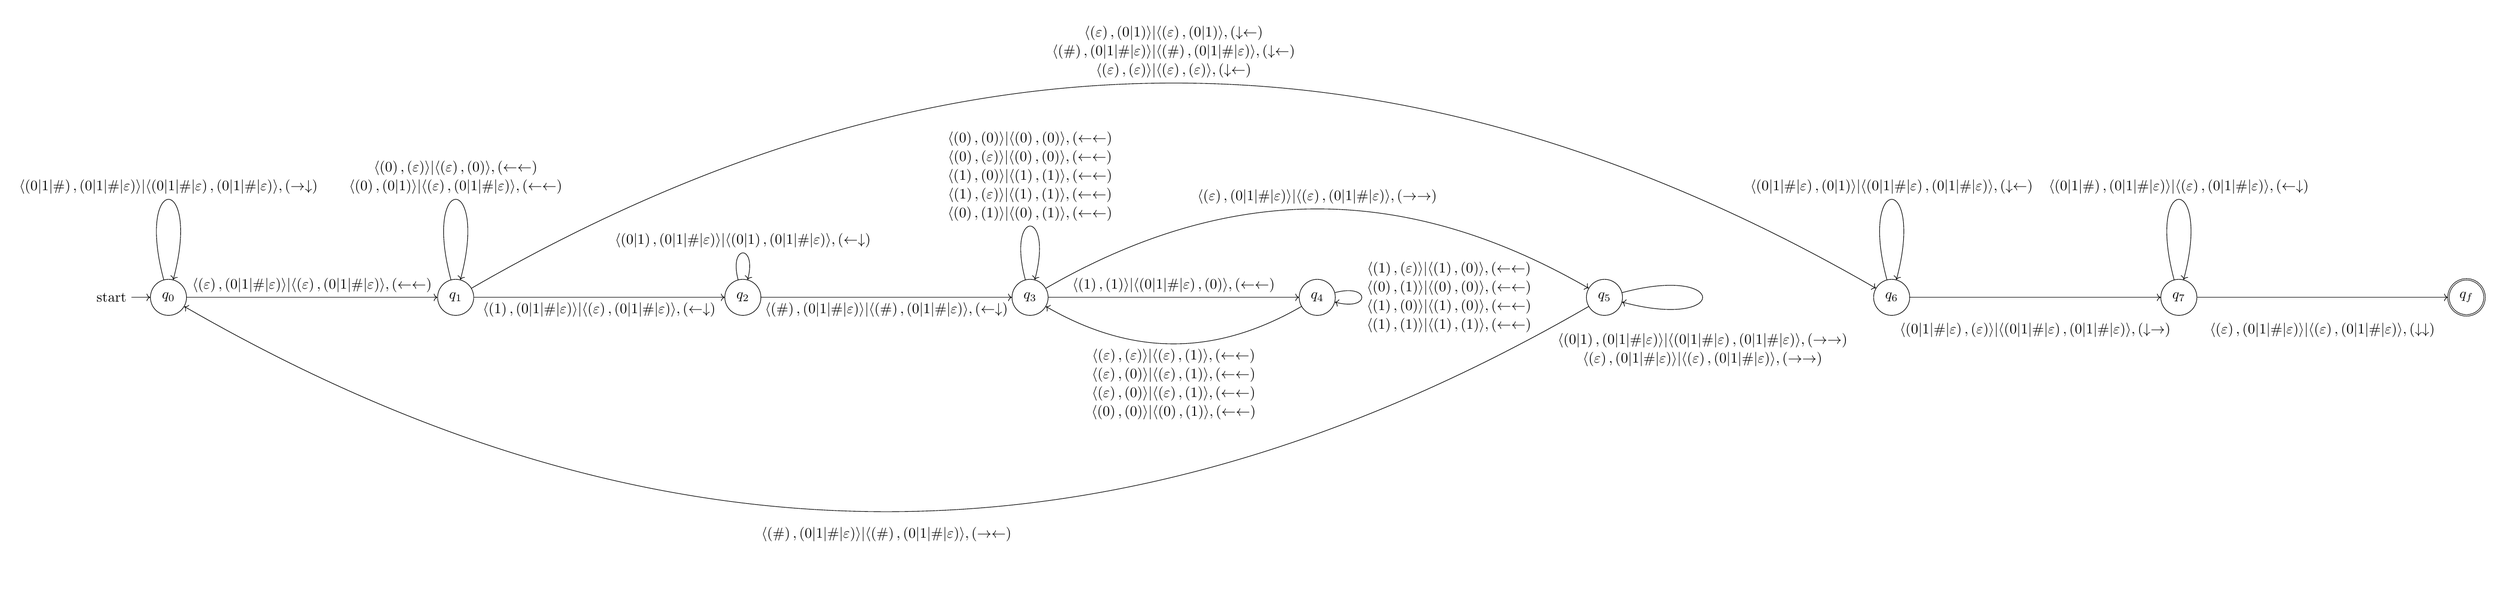
\begin{tikzpicture}[node distance=6.1cm]
  \node[state, initial] (q0) {$q_0$};
  \node[state] (q1) [right=of q0] {$q_1$};
  \node[state] (q2) [right=of q1] {$q_2$};
  \node[state] (q3) [right=of q2] {$q_3$};
  \node[state] (q4) [right=of q3] {$q_4$};
  \node[state] (q5) [right=of q4] {$q_5$};
  \node[state] (q6) [right=of q5] {$q_6$};
  \node[state] (q7) [right=of q6] {$q_7$};
  \node[state, accepting] (qf) [right=of q7] {$q_f$};

  \path[->] (q0) edge [loop above, looseness=30] node[above]{$\langle\left( 0 \vert 1 \vert \# \right),\left( 0 \vert 1 \vert \# \vert \varepsilon \right)\rangle \vert \langle\left( 0 \vert 1 \vert \# \vert \varepsilon \right),\left( 0 \vert 1 \vert \# \vert \varepsilon \right)\rangle, \left( \rightarrow\downarrow \right)$} (q0);
  \path[->] (q0) edge node[above]{$\langle\left( \varepsilon \right),\left( 0 \vert 1 \vert \# \vert \varepsilon \right)\rangle \vert \langle\left( \varepsilon \right),\left( 0 \vert 1 \vert \# \vert \varepsilon \right)\rangle, \left( \leftarrow\leftarrow \right)$} (q1);
  \path[->] (q1) edge [loop above, looseness=30] node[above]{\shortstack{
        $\langle\left( 0 \right),\left( \varepsilon \right)\rangle \vert \langle\left( \varepsilon \right),\left( 0 \right)\rangle, \left( \leftarrow\leftarrow \right)$\\
        $\langle\left( 0 \right),\left( 0 \vert 1 \right)\rangle \vert \langle\left( \varepsilon \right),\left( 0 \vert 1 \vert \# \vert \varepsilon \right)\rangle, \left( \leftarrow\leftarrow \right)$
      }} (q1);

  \path[->] (q1) edge node[below]{$\langle\left( 1 \right),\left( 0 \vert 1 \vert \# \vert \varepsilon \right)\rangle \vert \langle\left( \varepsilon \right),\left( 0 \vert 1 \vert \# \vert \varepsilon \right)\rangle, \left( \leftarrow\downarrow \right)$} (q2);
  \path[->] (q1) edge [bend left] node[above]{\shortstack{
        $\langle\left( \varepsilon \right),\left( 0 \vert 1 \right)\rangle \vert \langle\left( \varepsilon \right),\left( 0 \vert 1 \right)\rangle, \left( \downarrow\leftarrow \right)$\\
        $\langle\left( \# \right),\left( 0 \vert 1 \vert \# \vert \varepsilon \right)\rangle \vert \langle\left( \# \right),\left( 0 \vert 1 \vert \# \vert \varepsilon \right)\rangle, \left( \downarrow\leftarrow \right)$\\
        $\langle\left( \varepsilon \right),\left( \varepsilon \right)\rangle \vert \langle\left( \varepsilon \right),\left( \varepsilon \right)\rangle, \left( \downarrow\leftarrow \right)$
      }} (q6);

  \path[->] (q2) edge [loop above, looseness=10] node[above]{$\langle\left( 0 \vert 1 \right),\left( 0 \vert 1 \vert \# \vert \varepsilon \right)\rangle \vert \langle\left( 0 \vert 1 \right),\left( 0 \vert 1 \vert \# \vert \varepsilon \right)\rangle, \left( \leftarrow\downarrow \right)$} (q2);
  \path[->] (q2) edge node[below]{$\langle\left( \# \right),\left( 0 \vert 1 \vert \# \vert \varepsilon \right)\rangle \vert \langle\left( \# \right),\left( 0 \vert 1 \vert \# \vert \varepsilon \right)\rangle, \left( \leftarrow\downarrow \right)$} (q3);

  \path[->] (q3) edge [loop above, looseness=20] node[above]{\shortstack{
        $\langle\left( 0 \right),\left( 0 \right)\rangle \vert \langle\left( 0 \right),\left( 0 \right)\rangle, \left( \leftarrow\leftarrow \right)$ \\
        $\langle\left( 0 \right),\left( \varepsilon \right)\rangle \vert \langle\left( 0 \right),\left( 0 \right)\rangle, \left( \leftarrow\leftarrow \right)$\\
        $\langle\left( 1 \right),\left( 0 \right)\rangle \vert \langle\left( 1 \right),\left( 1 \right)\rangle, \left( \leftarrow\leftarrow \right)$\\
        $\langle\left( 1 \right),\left( \varepsilon \right)\rangle \vert \langle\left( 1 \right),\left( 1 \right)\rangle, \left( \leftarrow\leftarrow \right)$\\
        $\langle\left( 0 \right),\left( 1 \right)\rangle \vert \langle\left( 0 \right),\left( 1 \right)\rangle, \left( \leftarrow\leftarrow \right)$
      }}  (q3);

  \path[->] (q3) edge  node[above]{$\langle\left( 1 \right),\left( 1 \right)\rangle \vert \langle\left( 0 \vert 1 \vert \# \vert \varepsilon \right),\left( 0 \right)\rangle, \left( \leftarrow\leftarrow \right)$} (q4);
  \path[->] (q3) edge [bend left] node[above]{$\langle\left( \varepsilon \right),\left( 0 \vert 1 \vert \# \vert \varepsilon \right)\rangle \vert \langle\left( \varepsilon \right),\left( 0 \vert 1 \vert \# \vert \varepsilon \right)\rangle, \left( \rightarrow\rightarrow \right)$} (q5);

  \path[->] (q4) edge [bend left] node[below] {\shortstack{
        $\langle\left( \varepsilon \right),\left( \varepsilon \right)\rangle \vert \langle\left( \varepsilon \right),\left( 1 \right)\rangle, \left( \leftarrow\leftarrow \right)$\\
        $\langle\left( \varepsilon \right),\left( 0 \right)\rangle \vert \langle\left( \varepsilon \right),\left( 1 \right)\rangle, \left( \leftarrow\leftarrow \right)$ \\
        $\langle\left( \varepsilon \right),\left( 0 \right)\rangle \vert \langle\left( \varepsilon \right),\left( 1 \right)\rangle, \left( \leftarrow\leftarrow \right)$ \\
        $\langle\left( 0 \right),\left( 0 \right)\rangle \vert \langle\left( 0 \right),\left( 1 \right)\rangle, \left( \leftarrow\leftarrow \right)$
      }} (q3);

  \path[->] (q4) edge [loop right, looseness=10] node[right]{\shortstack{
        $\langle\left( 1 \right),\left( \varepsilon \right)\rangle \vert \langle\left( 1 \right),\left( 0 \right)\rangle, \left( \leftarrow\leftarrow \right)$\\
        $\langle\left( 0 \right),\left( 1 \right)\rangle \vert \langle\left( 0 \right),\left( 0 \right)\rangle, \left( \leftarrow\leftarrow \right)$\\
        $\langle\left( 1 \right),\left( 0 \right)\rangle \vert \langle\left( 1 \right),\left( 0 \right)\rangle, \left( \leftarrow\leftarrow \right)$\\
        $\langle\left( 1 \right),\left( 1 \right)\rangle \vert \langle\left( 1 \right),\left( 1 \right)\rangle, \left( \leftarrow\leftarrow \right)$
      }} (q4);

  \path[->] (q5) edge [loop right, looseness=30] node[below=0.75cm]{\shortstack{
        $\langle\left( 0 \vert 1 \right),\left( 0 \vert 1 \vert \# \vert \varepsilon \right)\rangle \vert \langle\left( 0 \vert 1 \vert \# \vert \varepsilon \right),\left( 0 \vert 1 \vert \# \vert \varepsilon \right)\rangle, \left( \rightarrow\rightarrow \right)$\\
        $\langle\left( \varepsilon \right),\left( 0 \vert 1 \vert \# \vert \varepsilon \right)\rangle \vert \langle\left( \varepsilon \right),\left( 0 \vert 1 \vert \# \vert \varepsilon \right)\rangle, \left( \rightarrow\rightarrow \right)$
      }} (q5);

  \path[->] (q5) edge [bend left] node[below=0.25cm]{$\langle\left( \# \right),\left( 0 \vert 1 \vert \# \vert \varepsilon \right)\rangle \vert \langle\left( \# \right),\left( 0 \vert 1 \vert \# \vert \varepsilon \right)\rangle, \left( \rightarrow\leftarrow \right)$} (q0);
  \path[->] (q6) edge [loop above, looseness=30] node[above]{$\langle\left( 0 \vert 1 \vert \# \vert \varepsilon \right),\left( 0 \vert 1 \right)\rangle \vert \langle\left( 0 \vert 1 \vert \# \vert \varepsilon \right),\left( 0 \vert 1 \vert \# \vert \varepsilon \right)\rangle, \left( \downarrow\leftarrow \right)$} (q6);
  \path[->] (q6) edge node[below=0.5cm]{$\langle\left( 0 \vert 1 \vert \# \vert \varepsilon \right),\left( \varepsilon \right)\rangle \vert \langle\left( 0 \vert 1 \vert \# \vert \varepsilon \right),\left( 0 \vert 1 \vert \# \vert \varepsilon \right)\rangle, \left( \downarrow\rightarrow \right)$} (q7);
  \path[->] (q7) edge [loop above, looseness=30] node[above]{$\langle\left( 0 \vert 1 \vert \# \right),\left( 0 \vert 1 \vert \# \vert \varepsilon \right)\rangle \vert \langle\left( \varepsilon \right),\left( 0 \vert 1 \vert \# \vert \varepsilon \right)\rangle, \left( \leftarrow\downarrow \right)$} (q7);
  \path[->] (q7) edge node[below=0.5cm]{$\langle\left( \varepsilon \right),\left( 0 \vert 1 \vert \# \vert \varepsilon \right)\rangle \vert \langle\left( \varepsilon \right),\left( 0 \vert 1 \vert \# \vert \varepsilon \right)\rangle, \left( \downarrow\downarrow \right)$} (qf);

\end{tikzpicture}
\end{document}